\section{Vorgehensmodelle}
Wie in Kapitel \ref{sec:einfuehrung} beschrieben, basieren alle Vorgehensmodelle auf wenigen klaren Regeln. Die bedeutendsten Modelle werden in diesem Kapitel genauer erläutert.

\subsection{Extreme Programming}
Extreme Programming (XP) ist eines der ältesten agilen Vorgehensmodelle und gibt Vorgaben für die Planung, das Management, das Quellcodedesign, das Testmanagement und die Programmierung eines Softwareprojekts. Dadurch wird XP sehr mächtig, aber auch anspruchsvoll für alle Beteiligten. \cite[S. 13]{bib:wolfRoock} \cite{bib:xp}

Einen Überblick über die Vorgehensweisen bei XP stellt die Abbildung \ref{fig:xppractices} dar. Der äußere Ring stellt die Planung da. Der mittlere Ring repräsentiert die Vorgehensweisen von Management und Design. Im inneren Ring sind die wichtigsten Punkte für das Testen und das Programmieren dargestellt.

\begin{figure}[h]
  \centering
  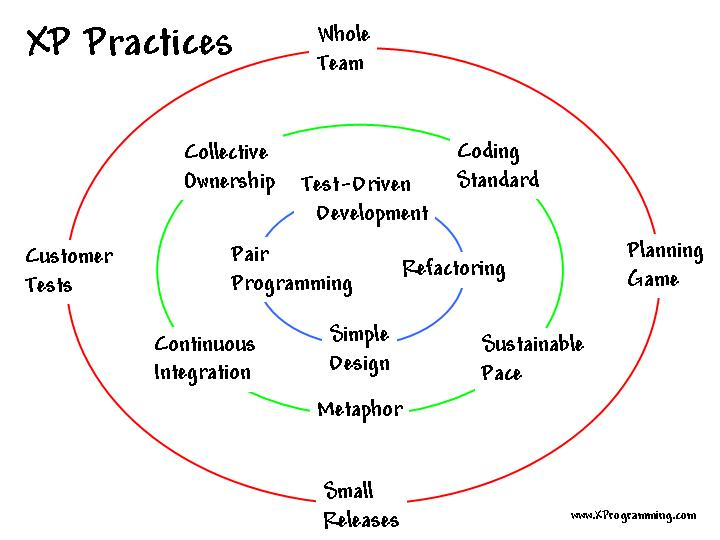
\includegraphics[width=0.8\textwidth]{images/xpCircles}
  \caption{Vorgehensweisen bei XP \cite{bib:xprogamming}}
  \label{fig:xppractices}
\end{figure}

\subsubsection{Planung}
Die Anforderungen an die Softwarelösung werden in sogenannten \emph{User Stories} festgehalten. Jede Story beschreibt eine Funktion, die der Kunde möchte. Eine solche User Story könnte wie folgt lauten:
\begin{quote}
Anzeige einer Druckvorschau beim Auswählen der Druckfunktion
\end{quote}
Danach wird ein \emph{Release-Plan} erstellt. In der Regel werden alle drei Monate Releases veröffentlicht. Bei der Erstellung des Plans legen die Entwickler grob fest, welche User Stories in welchem Release implementiert werden soll. Der Release-Plan ist jedoch stets veränderbar. Der Zeitraum zwischen zwei Releases wird wiederum in ein- bis drei-wöchige \emph{Iterationen} unterteilt. Zu Beginn jeder Iteration wählt der Kunde, die für ihn wichtigsten User Stories des kommenden Releases aus. Die Entwickler entwerfen, implementieren und testen die ausgewählten Stories innerhalb der Iteration. Die Stories können während einer Iteration nicht mehr verändert werden. Am Ende jeder Iteration muss das Programm lauffähig sein, auch wenn noch wichtige Funktionen fehlen.

\subsubsection{Management}
Auch für das Management eines Softwareprojekts sind bei XP klare Regeln definiert. Täglich gibt es ein Meeting, bei dem jeder Entwickler kurz sagt, was er am Vortag getan hat, was er heute tun wird und welche Probleme er sieht. Eine weitere wichtige Regel ist, dass ein Entwickler nicht länger arbeiten darf, als er auf unbefristete Zeit leisten kann. Normalerweise sind dies acht Stunden pro Tag. Überstunden sind nicht gern gesehen. Des Weiteren soll jeder Entwickler in den gesamten Prozess eingebunden sein und immer über den Gesamtstand des Projektes informiert sein. Außerdem sollen Entwickler immer wieder mit anderen Aufgaben betraut werden. Damit soll vermieden werden, dass sie den Anschluss zum technologischen Geschehen verlieren. Aus dem selben Grund soll den Entwicklern auch genügend Freiraum gegeben werden, um auch während eines Projekts sich mit technischen Neuerungen zu befassen.

\subsubsection{Quellcodedesign}
Da im Gegensatz zu klassischen Vorgehensmodellen die endgültige Architektur der Softwarelösung während der Programmierung noch nicht klar ist, sind beim Design einige Regeln zu beachten. Die wichtigste ist hier die Einfachheit. Der Quellcode ist so einfach wie möglich zu halten. Es sollen keine unnötigen Funktionen implementiert werden und es ist so zu programmieren, dass jeder aus dem Team den Quellcode verstehen kann. Des Weiteren soll immer wenn es sinnvoll ist, refactort werden.

\subsubsection{Testmanagement}
Bei Extreme Programming wird testgetrieben entwickelt. Das heißt, der Unit-Test einer Funktion wird vor der Funktion selbst implementiert. Diese Art der Programmierung zwingt den Programmierer zu einer genaueren Überlegung, was die Funktion erledigen soll und welche Grenzfälle dabei auftreten können. Und dabei stellt das \emph{Test First} genannte Prinzip gleichzeitig sicher, dass es eine komplette Testabdeckung gibt. Die Unit-Tests werden mehrmals täglich ausgeführt. Zur weiteren Verbesserung der Qualität werden die Änderungen der Entwickler mehrfach am Tag in die gemeinsame Quellcodebasis integriert und kompiliert. Dieser Integrationstest stellt sicher, dass die einzelnen Teilkomponenten korrekt miteinander kommunizieren können. Noch eine Stufe abstrakter ist der \emph{Acceptance Test}. Dies ist ein Black-Box-Test, der nach jeder Iteration vom Kunde durchgeführt wird. Jeder Fehler, der vom Kunde gemeldet und von den Entwicklern behoben wurde, muss mit einem Unit-Test abgedeckt werden um ihn zukünftig zu vermeiden.

\subsubsection{Programmierung}
Die auffälligste Unterscheidung von XP zu klassischen Vorgehensmodellen ist das \emph{Pair Programming}. Es sitzen immer zwei Entwickler vor einem Rechner und einer Tastatur und programmieren gemeinsam. Dabei wechseln sie sich regelmäßig beim Schreiben des Codes ab. Dies soll bei geringem Zeitverlust eine starke Qualitätssteigerung mit sich bringen. Weniger auffällig, aber trotzdem wichtig ist die Regel, dass jeder Entwickler das Recht hat jede Codezeile des Projektes zu ändern. Das heißt, wenn ihm Fehler oder Unstimmigkeiten auffallen, kann er diese gleich beheben.

\subsection{Scrum}
\label{ch:scrum}
Laut einer Studie von 2010 von \emph{Forrester Research} ist Scrum die verbreitetste agile Methode. So verwendeten ca. 11 \% der befragten IT-Fach\-kräfte das wohl bekannteste agile Vorgehensmodell. \cite{bib:ane} Scrum bietet deutlich weniger Regeln als Extreme Programming und gilt somit als verhältnismäßig leicht einzusetzen. 

\subsubsection{Rollenverteilung}
Im Zentrum von Scrum steht ein hochmotiviertes und selbstgesteuertes Entwicklerteam. Die Rollenverteilung von klassischen Vorgehensmodellen wird grundlegend verändert. Der Produktmanager wird zum Product Owner. Der Teamleiter wird zum Scrum Master. Und das Team, zu dem alle Entwickler gehören, bekommt deutlich mehr Verantwortung.

\begin{description}
\item Product Owner\\
Er bringt die Produktvision mit sich und ist verantwortlich für das Produkt. Dabei definiert er die Anforderungen, priorisiert sie und kontrolliert die Ergebnisse. Zusätzlich behält er das Budget und die Wirtschaftlichkeit im Blick. Wichtig: Der Product Owner gibt dem Team keine Zeitvorgaben.

\item Scrum Master\\
Der Scrum Master sorgt für die Einhaltung des Entwicklungsprozesses und den Scrum-Regeln. Hierzu schützt er das Team auch vor Störungen von außen und beseitigt organisatorische Probleme. Wichtig: Der Scrum Master vergibt keine Aufgaben.

\item Team\\
Das Team steht im Mittelpunkt des Entwicklungsprozesses. Es entscheidet selbst wann es welche Aufgaben erledigt. Verantwortung übernimmt das Team für das Zeit-, Qualitäts- und Dokumentationsmanagement.
\end{description}

\subsubsection{Prozess}
Die Abbildung \ref{fig:scrum} stellt das Vorgehen bei Scrum dar. Zu Beginn des Projekts stellt der Product Owner das \emph{Product Backlog} auf, in dem die Anforderungen des Produkts mit User Stories beschrieben werden. Das Product Backlog kann jederzeit vom Product Owner mit weiteren Anforderungen erweitert werden. Jede Anforderung bekommt vom Product Owner eine Priorität, die sich auch im Laufe des Projekts verändern kann. Das priorisierte Product Backlog stellt der Product Owner im \emph{Sprint Planning Meeting} dem Team vor. Beim Sprint Planning Meeting wählt das Team so viele User Stories aus dem Product Backlog aus, wie es denkt während der nächsten Iteration (\emph{Sprint} abarbeiten zu können. Die User Stories teilt das Team in einzelne Aufgaben auf und hält sie im \emph{Sprint Backlog} fest. Das Sprint Backlog darf während einer Iteration nicht verändert werden.

\begin{figure}[h]
  \centering
  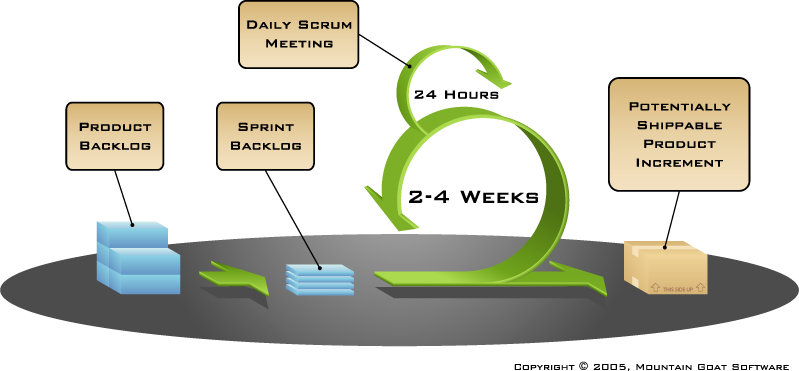
\includegraphics[width=1\textwidth]{images/scrum}
  \caption{Prozessüberblick bei Scrum \cite{bib:mountaingoat}}
  \label{fig:scrum}
\end{figure}

Nach dem Meeting beginnt der Sprint. Ein Sprint stellt eine Iteration von zwei bis vier Wochen dar und wird immer wieder durchlaufen. Während des Sprints findet täglich ein \emph{Daily Scrum Meeting} statt an dem das Team und der Scrum Master teilnehmen. Dieses ist gleich aufgebaut wie das tägliche Meeting beim Extreme Programming. Die Dauer des Meetings legt der Scrum Master in der Regel auf 15 Minuten fest und hält dies auch ein. Jeder Teilnehmer bespricht kurz die folgenden drei Dinge:
\begin{itemize}
  \item Was habe ich gestern gemacht? 
  \item Was steht heute auf dem Plan? 
  \item Und welche Probleme habe oder sehe ich?
\end{itemize}
Im Sprint Backlog wird der tägliche Fortschritt festgehalten. Dadurch entsteht ein immer aktuelles Burn-Down Diagramm (Abbildung \ref{fig:burndown}), das den Fortschritt des Sprints übersichtlich darstellt. 

\begin{figure}[h]
  \centering
  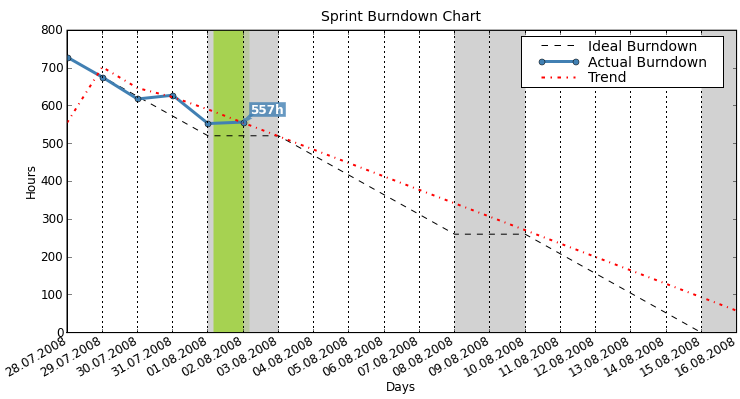
\includegraphics[width=1\textwidth]{images/burndown}
  \caption{Burn-Down Diagramm eines Sprints \cite{bib:agilo}}
  \label{fig:burndown}
\end{figure}

Am Ende des Sprints muss eine lauffähige Version des Programms verfügbar sein, die dem Product Owner im \emph{Sprint Review Meeting} präsentiert wird. Zusätzlich gibt es noch das \emph{Sprint Retrospective Meeting}, an dem über den vergangen Sprint reflektiert wird um über Veränderungen eine Verbesserung des Prozesses zu erzielen.

\subsubsection{Scrum Anti-Pattern}
Marion Eickmann schreibt, dass Scrum nur dann funktioniert, wenn auch alle Beteiligten sich an die Regeln halten: ``Alle Beteiligten müssen sich an das neue Vorgehen gewöhnen und sind unsicher was zu tun ist, wenn Unerwartetes geschieht. Solche Schwierigkeiten führen häufig dazu, `bekannte' Mechanismen `nur für den Fall' anzuwenden, statt das Problem nach Scrum-Art zu lösen.'' \cite[S. 84]{bib:ix2010}. So führt sie in ihrem Artikel mehrere bekannte Scrum Anti-Pattern auf, die es gilt zu vermeiden. Die wichtigsten seien hier aufgezählt:
\begin{itemize}
  \item Der Scrum Master weist Tasks zu und zerstört so das sich selbst steuernde und organisierende Team
  \item Der Sprint wird von außen gestört. Es werden neue Aufgaben eingefügt oder Änderungen an den gewählten (committed) User Stories vorgenommen.
  \item Es finden keine Review Meetings statt
  \item Es findet keine Retrospective statt
  \item Es gibt keine regelmäßigen Daily Standup Meetings
  \item Der Product Owner hat keine ausreichende Kompetenz und nimmt seine Rolle nicht war
  \item Meetings sind nicht Time-Boxed
  \item Statt Funktionen werden Aktivitäten erfasst
\end{itemize} 

\subsubsection{Verknüpfung mit anderen Methoden}
Da Scrum lediglich Vorgaben für die Planung und das Management eines Softwareprojekts macht, wird es oftmals mit anderen Vorgehensmodellen kombiniert. So können zum Beispiel die Punkte Quellcodedesign, Testmanagement und Programmierung von Extreme Programming übernommen werden. Das kombinierte Vorgehensmodell hat zwar viele Regeln, die es gilt einzuhalten, aber deckt den kompletten Softwareentwicklungsprozess ab.

\subsection{Software Kanban}
Software Kanban ist die jüngste der hier vorgestellten Methoden und unterscheidet sich auch stark ihnen. So gibt Software Kanban nicht vor wie man ein Projekt durchführt, sondern lediglich wie man den Prozess von einer klassischen Vorgehensweise in eine Agile umwandelt (\emph{Change Management Methode}). \cite[S. 14]{bib:wolfRoock} Dabei wird versucht den Entwicklungsprozess Schritt für Schritt zu verbessern, statt einen radikalen Schnitt wie bei Scrum oder XP zu wagen. Dies minimiert die Widerstände der einzelnen Beteiligten gegenüber großen Veränderungen. \cite{bib:ix2011}

\subsubsection{Grundprinzipien}
David J. Anderson \cite{bib:anderson}, der Erfinder von Software Kanban, definiert drei Grundprinzipien für die Methode:
\begin{itemize}
  \item Beginne dort, wo du dich im Moment befindest
  \item Komme mit den anderen überein, dass inkrementelle, evolutionäre Veränderungen angestrebt werden
  \item Respektiere den bestehenden Prozess sowie die existierenden Rollen, Verantwortlichkeiten und Berufsbezeichnungen
\end{itemize}

Durch das erste Grundprinzip entstehen viele verschiedene Implementierungen der Methode. So kann Software Kanban an ein bestehendes Wasserfallmodell gekoppelt werden oder auch eine bestehende Implementierung des V-Modells langsam verändern und verbessern.

Des Weiteren definiert Anderson fünf Kerneigenschaften von Software Kanban, die im folgenden näher erläutert werden.

\subsubsection{Visualisierungen}
Als erster Schritt in Software Kanban wird der aktuelle Entwicklungsprozess visualisiert. Es bietet sich ein Whiteboard mit den einzelnen Prozessschritten als Spalten dargestellt an. Ein solches Whiteboard ist in Abbildung \ref{fig:kanbanBoard} dargestellt. Typische Prozessschritte sind zum Beispiel:
\begin{itemize}
  \item Idee/Bestellung (Backlog)
  \item Eingeplant
  \item Entwicklung
  \item Test
  \item Auslieferung
  \item Produktiv
\end{itemize}

Zu jeder Spalte sind eine oder mehrere Personen zugeordnet. Wenn es bei der Vorgängermethode zum Beispiel auch Softwarearchitekten gab, muss eine Spalte \emph{Design} hinzugefügt werden. Die Spalten \emph{Entwicklung} und \emph{Test} werden nochmals unterteilt in \emph{laufend} und \emph{erledigt}. 

\begin{figure}[h]
  \centering
  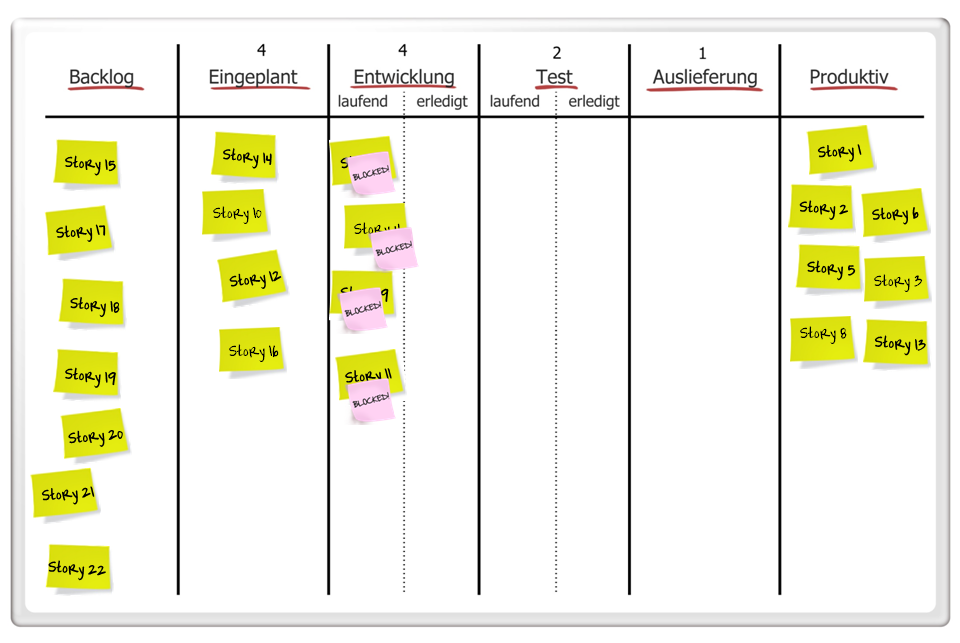
\includegraphics[width=1\textwidth]{images/kanbanBoard}
  \caption{Visualisierung eines Entwicklungsprozesses in Software Kanban \cite{bib:roock}}
  \label{fig:kanbanBoard}
\end{figure}

Die einzelnen Anforderungen (\emph{Ticket}) an das Softwareprodukt werden auf Haftnotizen oder Karteikarten geschrieben, mit einer Priorität versehen und in die Spalte \emph{Backlog} geheftet. Jede Anforderung durchläuft nun den gesamten Prozess, wobei immer notiert wird, wann die Anforderung in welcher Spalte aufgenommen wurde.

Ein kleiner Bruch mit der Vorgängermethode stellt nun das \emph{Pull-Prinzip} dar. Wer eine Aufgabe erledigt hat, darf sich in der Vorgängerspalte eine neue Anforderung nehmen und abarbeiten. Eine Überbelastung der Beteiligten wird damit vermindert, da jeder selbst entscheidet wie viel Arbeit er auf sich nimmt und in welcher Geschwindigkeit er diese bewältigt.

\subsubsection{Begrenzungen}
Für jede Spalte wird nun ein \emph{Work in Progress-Limit} (\emph{WiP-Limit}) festgelegt. Es bestimmt wie viel Tickets pro Prozessschritt maximal gleichzeitig bearbeitet werden dürfen. Dadurch minimieren sich Zeitverlust und Flüchtigkeitsfehler durch häufige Kontextwechsel. Außerdem werden Engpässe schneller sichtbar. Wenn zum Beispiel die Testabteilung ständig am Limit arbeitet, sollten hier eventuell mehr Personen eingesetzt werden.
Die WiP-Limits werden wie in Abbildung \ref{fig:kanbanBoard} zu jeder Spalte geschrieben.

\subsubsection{Messungen}
Eine weitere Kerneigenschaft von Software Kanban ist die ständige Erstellung von Metriken. Hierbei sind zwei Messungen besonders wichtig:
\begin{description}
  \item Lead Time\\ Durchlaufzeit einer Anforderung vom Backlog bis zur Auslieferung
  \item Cycle Time\\ Reine Entwicklungszeit ohne Wartezeiten
\end{description}
Weitere Messungen sind unter anderem \emph{Durchsatz}, \emph{Fehlerrate} und \emph{Termintreue}. Durch die Darstellung der Metriken werden Engpässe und Verbesserungsmöglichkeiten sichtbar. Auch die Tickets werden überwacht und z.B. als Cumulative Flow Chart (Abbildung \ref{fig:kanbanChart}) dargestellt.

\begin{figure}[h]
  \centering
  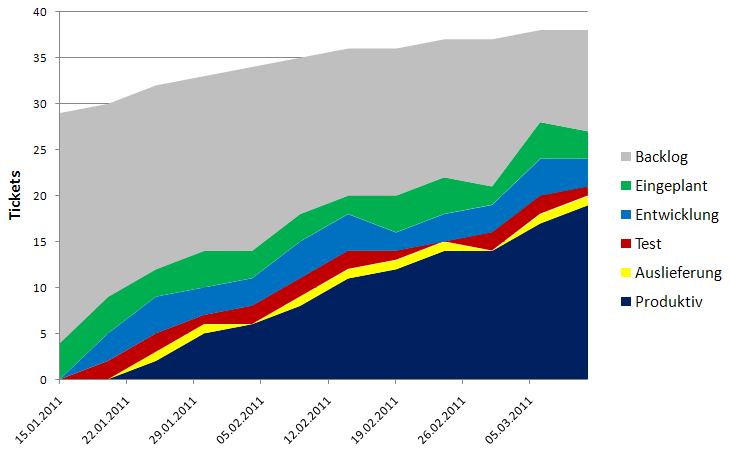
\includegraphics[width=1\textwidth]{images/kanbanChart}
  \caption{Cumulative Flow Chart der Tickets}
  \label{fig:kanbanChart}
\end{figure}

\subsubsection{Prozessregeln}
Um die Vorgehensweise für alle Beteiligten transparent darzustellen werden alle Regeln festgehalten. Es bietet sich an alle Prozessregeln direkt neben dem Whiteboard anzubringen. Beispiele für solche Regeln sind:
\begin{itemize}
  \item Wodurch kommen Tickets in das Backlog?
  \item In welcher Reihenfolge werden Tickets abgearbeitet?
  \item Wann dürfen WiP-Limits gebrochen werden
  \item Wie werden Bugs in dem Prozess behandelt?
\end{itemize}

\subsubsection{Verbesserungen}
Die fünfte Kerneigenschaft von Software-Kanban ist die kontinuierliche Verbesserung. Hierzu können nach und nach weitere Merkmale von anderen agilen Vorgehensmodellen wie Scrum und XP übernommen werden. So kann ein tägliches Stand-Up-Meeting die Kommunikation erhöhen. Pair Programming erhöht die Qualität. Test First verbessert ebenfalls die Qualität. 

Wichtig bei der Einführung der neuen Merkmale ist die Akzeptanz bei allen Beteiligten. Wenn der Verbesserungsprozess zu schnell durchgeführt wird, werden einige Beteiligte sich gegen die Veränderungen wehren und den gesamten Prozess stören. Ob eine Veränderung auch eine Verbesserung der Situation bedeutet kann mit den erstellten Metriken überprüft werden. Im Notfall sollte die Veränderung auch wieder rückgängig gemacht werden können.

\subsection{Ergebnisse}
Als Paradebeispiele für agiles Vorgehen gelten Extreme Programming und Scrum, welche auch zu den beliebtesten Methoden zählen. Sie geben den Entwicklern und Projektbeteiligten wenige klare Regeln an die Hand und steigern dadurch Flexibilität, Effizienz und Transparenz. \cite[S. 28 f.]{bib:wolfRoock} Wenn die Widerstände gegen eine Umstellung auf eine der Methoden zu groß sind, kann die Change-Management-Methode Software Kanban einen sanften Einstieg in die agile Softwareentwicklung zu ermöglichen. Hier wird eine evolutionäre Umstellung der bestehenden Strukturen durchgeführt.